\chapter{The Origin of Algorithms}\label{ch:1hkdh,kxch,.kdh,}
\section{Matematician from Uzbekistan}

\begin{figure}[h]
    \centering
    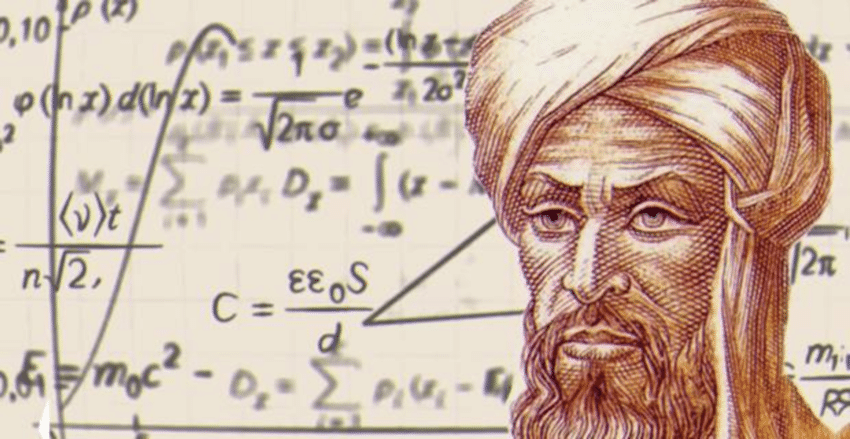
\includegraphics[scale=0.4]{figures/alkhwarizmi.png}
    \caption{Abu Abdullah Muhammad ibn Musa Al-Khawarizmi}
    \label{fig:gp}
\end{figure}

The term algorithm got its name from the Persian astronomer and mathematician, Abu Abdullah Muhammad ibn Musa Al-Khawarizmi (780 AD).\\
He was from a Persian city known as Khwarizm, found in present-day Uzbekistan.\\
Al-Khwarizmi wrote many important mathematical books that were later translated into Latin.\\
It was his book on Arabic-Hindu numerals and arithmetic, called Al-Khw?rizm? On the Hindu Art of Reckoning, later Latinized as Algoritmi de numero Indorum that gave the word algorithm to the Western world. \\

\pagebreak

\section{First Algorithm}

\begin{figure}[h]
    \centering
    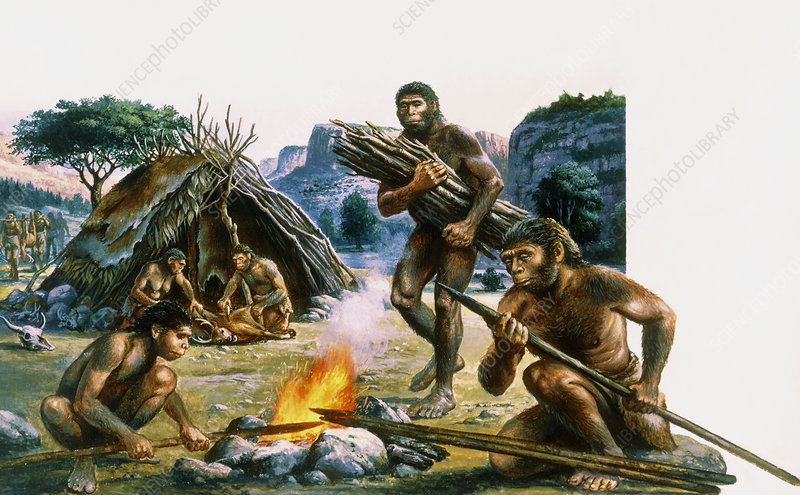
\includegraphics[scale=0.4]{figures/homo_erectus.jpg}
    \caption{Homo Erectus}
    \label{fig:gp}
\end{figure}

Generally, the existence of algorithms as long as human history. As an example, the creation of the first artificial fire in the Wonderwerk Cave of South Africa, millions of years ago by Homo Erectus, constitutes our first evidence of the use of algorithms. However, most historians hold the view that the Babylonian clay tablets (1600-1800 BC) are the world's first known algorithm. The Babylonians had developed a numerical system using cuneiform numerals to count and they preserved those calculations on tablets. \\ 

\begin{figure}[h]
    \centering
    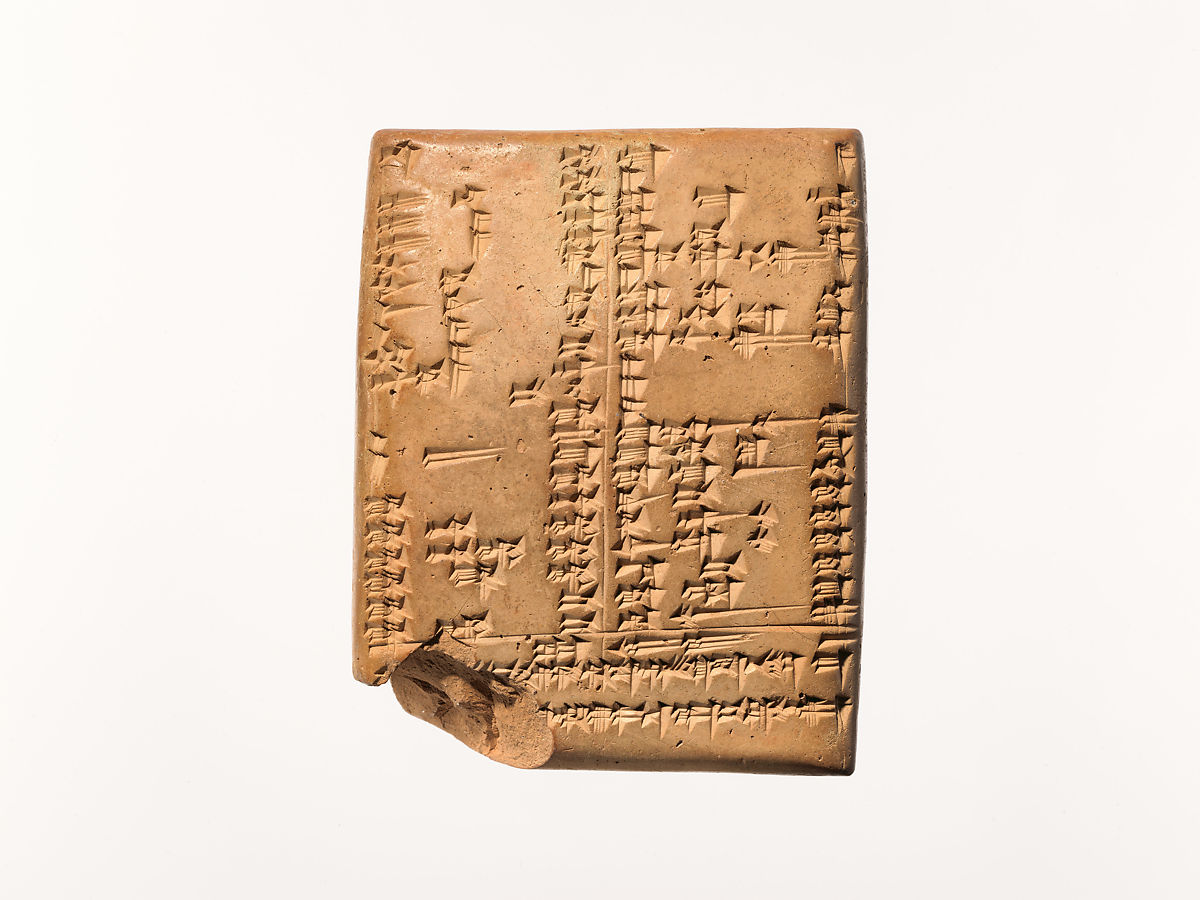
\includegraphics{figures/tablet.jpg}
    \caption{Cuneiform tablet}
    \label{fig:gp}
\end{figure}

Although we can find instances of algorithms in Euclidean mathematics,\\
Archimedes approximation of Pi, or Eratosthenes calculation of prime numbers, it was the work of George Boole in developing what is known as Boolean algebra, in 1847, that set the basis for computer logic today. Boole developed a system of logic to make calculations that used true and false values as basic units (binary algebra). This system would later be represented in digital form by zeros and ones or binary digits in low-level programming languages. \\ 

\section{Computing machine}

Some decades later, Alan Turing came up with a mathematical model of a hypothetical computing machine. It used squares that contained symbols or binary digits in an infinitely long tape. This tape served as storage space for the data in the squares, computer memory. It has a head or needle that can move to the right or left of each square to read, write, or erase the symbol within it, the basis for CRUD (Create, Read, Update, and Delete) operations in programming. Using this system this machine could simulate any algorithm, regardless of its complexity!
Mathematicians and computer scientists continued adding to Turing's concept of a computing machine to advance technology to what we know today. Algorithms then evolved from binary operations to high-level, more human-friendly, programming languages like C++, Java, and etc. Because they allow creating efficient, error-free software applications, they will continue to be important in the foreseeable future. \\ 


\begin{figure}[h]
    \centering
    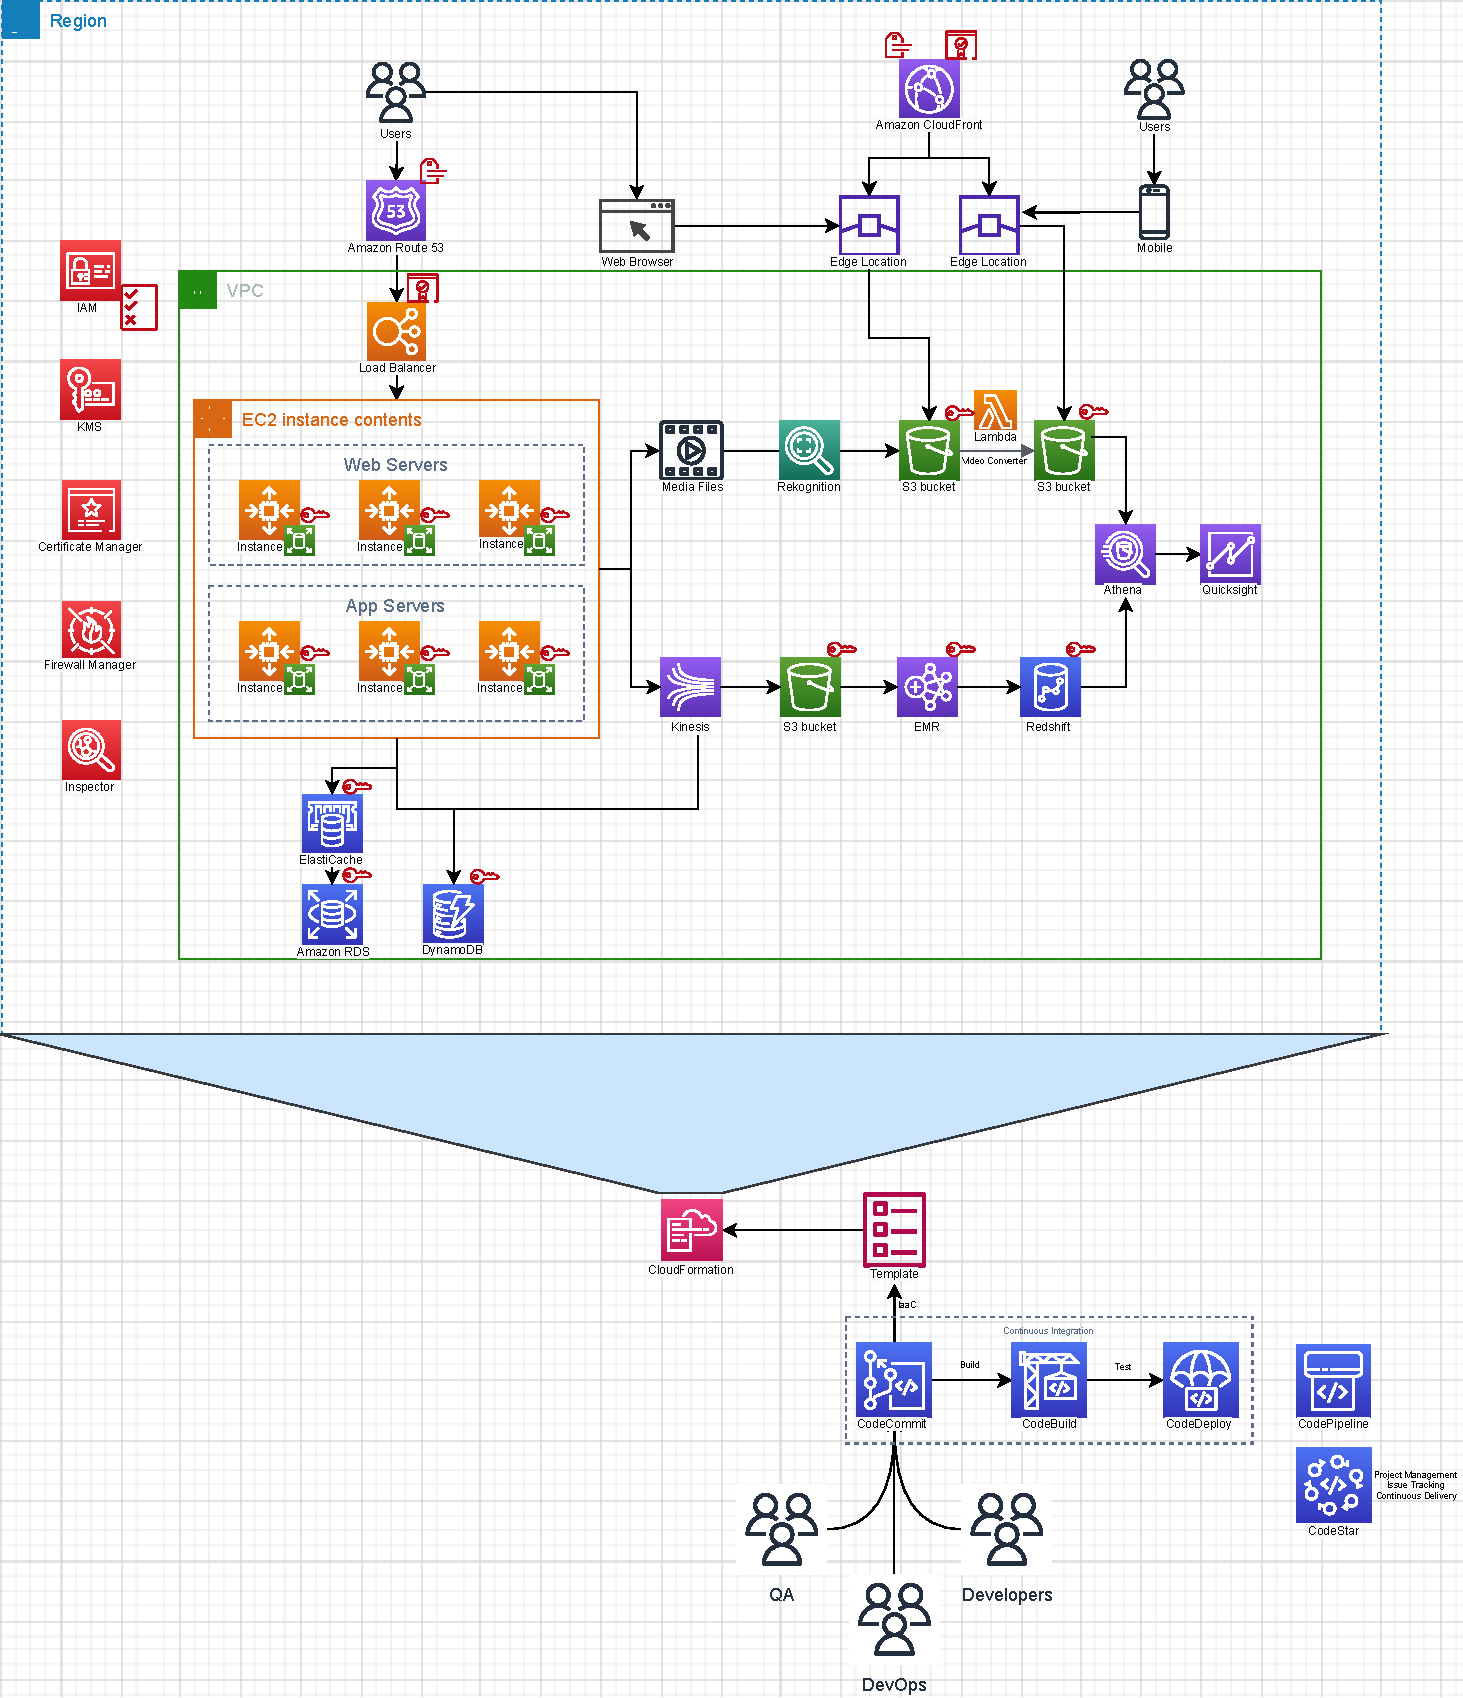
\includegraphics[scale=0.7]{figures/sys.pdf}
    \caption{System Design}
    \label{fig:gp}
\end{figure}
